\documentclass[11pt,a4paper]{article}
\pdfoutput=1
%vons grund
\usepackage[utf8]{inputenc}
\usepackage[T1]{fontenc}
\usepackage[swedish]{babel} %OBS! Se till att vi får rätt språk.
\usepackage{amsmath}
\usepackage{lmodern}
\usepackage{units}
\usepackage{icomma}
\usepackage{color}
\usepackage{graphicx}
\usepackage{bbm}
\newcommand{\N}{\ensuremath{\mathbbm{N}}}
\newcommand{\Z}{\ensuremath{\mathbbm{Z}}}
\newcommand{\Q}{\ensuremath{\mathbbm{Q}}}
\newcommand{\R}{\ensuremath{\mathbbm{R}}}
\newcommand{\C}{\ensuremath{\mathbbm{C}}}
\newcommand{\rd}{\ensuremath{\mathrm{d}}}
\newcommand{\id}{\ensuremath{\,\rd}}
\usepackage{hyperref}
\usepackage{float}
\usepackage{todonotes}
\usepackage{epstopdf}
\usepackage{verbatim}


%%%%%%%%%%%%%%%%%%%%%%%Egna tillägg%%%%%%%%%%%%%%%%%%%%%%%
%%För att figurtext i underfigurer
\usepackage{subcaption} 
%%För att få referenser 'på svenska'
\usepackage[fixlanguage]{babelbib}
\selectbiblanguage{swedish}
%\renewcommand\btxauthorcolon{:}
%%Partiell derivata
\newcommand{\pd}{\ensuremath{\partial}}
%%Följer ISO-8601 oberoende av språk.
\usepackage{datetime} 
\newdateformat{specialdate}{\THEYEAR-\twodigit{\THEMONTH}-\twodigit{\THEDAY}}
%%Göra grader Celcius
\newcommand{\degC}{\ensuremath{\,^\circ\mathrm{C}}}
%%Figurreferenser
\newcommand{\figref}{\figurename~\ref}
%%Tabellreferenser
\newcommand{\tabref}{\tablename~\ref}
%%För att själv bestämma marginalerna. 
\usepackage[
%            top    = 3cm,
%            bottom = 3cm,
%            left   = 3cm, right  = 3cm
]{geometry}

\usepackage{rotating} %För att ha figurer på snedden
\usepackage{pdfpages}

\usepackage{tocstyle}
\usetocstyle{standard}
%\usetocstyle{nopagecolumn}
%\settocstylefeature[-1]{entryhook}{\hfil}%centering part entry
\settocstylefeature[-1]{pagenumberbox}{\csname @gobble\endcsname}%no page numbers for part

\usepackage[nottoc]{tocbibind} %Puts an 'Reference' entry in the ToC.

\begin{document}

\title{Två metoder för bestämning av tyngdaccelerationen samt mätning av Newtons gravitationskonstant med Cavendishs experiment}
\author{Johan Runeson\\
\href{mailto:johanru@student.chalmers.se}{\nolinkurl{johanru@student.chalmers.se}}
\and 
Andréas Sundström \\ 
\href{mailto:andsunds@student.chalmers.se}{\nolinkurl{andsunds@student.chalmers.se}}
}
\date{\specialdate\today}
\begin{titlepage}


\maketitle


%Kanske lite för stort sammandrag. 
\renewcommand\abstractname{Sammandrag}
\begin{abstract}
\noindent I denna rapport beskrivs två olika sätt att mäta tyngdaccelerationen $g$ och ett sätt att mäta Newtons gravitationskonstant $G$. Tyngdaccelerationen mäts först och främst med en reversionspendel, som är en väl beprövad metod, för att erhålla maximal noggrannhet. Huvudprincipen bakom det andra sättet att mäta $g$ bygger på att ytan till en vätska i en roterande skål kommer att bilda en paraboloid. Denna metod att mäta $g$ verkar inte ha studerats i högre utsträckning tidigare. Resultaten från de två metoderna att mäta $g$ överensstämde med varandra. Det noggrannaste resultatet var från mätningen med reversionspendeln och gav $g=\unit[9,823\pm 0,005]{m\,s^{-2}}$. Mätningen med den roterande vätskan gav $g=\unit[9,78\pm 0,13]{m\,s^{-2}}$. Vidare behandlar även denna rapport mätningen av $G$ med en uppställning baserad på Cavendishs experiment. Resultatet från dessa mätningar gav $G=\unit[(8\pm2)\times 10^{-11}]{N\,m^2\,kg^{-2}}$. Detta är inte helt överensstämmande med tidigare kända värden på $G$, men det ligger inom felmarginalen för dessa mätningar. 

\end{abstract}


\renewcommand\abstractname{Abstract}
\begin{abstract}
\noindent In this report two methods of measuring Earth's acceleration of gravity $g$ and a way to measure Newton's gravitational constant are presented. The acceleration of gravity was first and foremost measured using Kater's pendulum, which is a well tested method, to obtain a maximum of accuracy. The main principle of the other method of measuring $g$ is that a rotating bowl of liquid will form a parabola. It seems as if this method haven't been thoroughly investigated before. The results from the two methods of measuring $g$ were in agreement with each other. The most accurate measurement was with the Kater pendulum and it was $g=\unit[9.823\pm 0,005]{m\,s^{-2}}$. The measurement with the rotating liquid gave $g=\unit[9.78\pm 0,13]{m\,s^{-2}}$. This report will furthermore deal with the measurement of $G$ using an apparatus based on the Cavendish experiment. The results from these measurements were $G=\unit[(8\pm2)\times 10^{-11}]{N\,m^2\,kg^{-2}}$. This is not in ful agreement with the known values of $G$, but it's within the margin of error of these measurements. 

\end{abstract}
\pagenumbering{roman}

\newpage
%\newgeometry{top=4cm}
\renewcommand{\contentsname}{Innehållsförteckning}
\tableofcontents
\end{titlepage}

\pagenumbering{arabic}
\setcounter{page}{1}

\section{Inledning}
%Redan på 1600-talet satt Newton med sitt äpple och funderade över gravitationen. Man visste att två 
Galileo brukar tillskrivas att ha visat att alla objekt faller lika fort oavsett vad för objekt de är om man bortser från luftmotstånd. Det visar sig dessutom att två fritt fallande objekt accelererar med en konstant acceleration -- \emph{tyngdaccelerationen}. 

Att mäta jordens tyngdacceleration, $g$, är ett vanligt skolexperiment som brukar göras på gymnasienivå. En vanlig metod är att använda en plan pendel och från det få ett resultat med en relativ osäkerhet på $10^{-2}$ som bäst. Där använder man sig oftast av enklast möjliga modell för en sådan pendel, nämligen den matematiska pendeln. Och för en så låg noggrannhet är den oftast tillfredsställande, men ska $g$ mätas med med högre noggrannhet krävs andra och bättre modeller.

Med introduktionen av en pendelmodell som bygger på rörelsemängdsmoment och tröghetsmoment -- den \emph{fysikaliska pendeln} -- kan pendelns rörelse beskrivas mycket noggrannare. Den fysikaliska pendeln kräver dock att man känner till pendelns rörelsemängdsmoment som kan vara mycket svårt att mäta. År 1817 uppfann Henry Kater en pendel som gjorde det möjligt att bestämma $g$ utan att veta vad pendeln har för tröghetsmoment\cite{wiki:katerpendel}. Metoden går ut på att finna två olika upphängningspunkter på varsin sida om masscentrum som ger samma svängningsfrekvens -- pendeltypen har därför fått namnet \emph{reversionspendel}.

I denna rapport används en reversionspendel enligt Katers idé för att mäta tyngdaccelerationen med en relativ noggrannhet på $5\times10^{-4}$. För att uppnå detta används flera moderna instrument samt matematiska korrektioner för bland annat pendelns utslagsvinkel och dämpning. 

%De flesta sätt att mäta $g$ på brukar involvera pendlar av något slag, oftast för att pendlar är bland de enklaste sätten. Det finns dock problem med pendlar som beskrivits ovan. 
En annan metod som skulle kunna göras på gymnasienivå är att mäta vattenytan i en roterande skål med vatten. Det går enkelt att med fysik från gymnasiet härleda att formen för vattenytan kommer att bli en paraboloid vars form helt bestäms av $g$ och rotationshastigheten. Detta är samma form som parabolantenner för till exempel satellit-TV har.

I denna rapport utnyttjas att paraboloider fokuserar plant infallande ljus till en punkt, oavsett var ljuset träffar parabolen, för att bestämma dess form. Denna fokalpunkt är nämligen entydigt bestämd av paraboloidens form. Detta är en enkel metod, både teoretiskt och praktiskt, för att bestämma $g$. 

Det finns visserligen många teoretiska beskrivningar av formen hos vattenytan i en roterande vattenskål, men ytterst få praktiska undersökngar av detta fenomen. En snabb sökning efter publicerat material inom området gav i huvudsak två resultat. Dels \v{S}abatka och Dv\v{o}rák\cite{Sabatka2010} som med ett system av stavar bekräftat att vattenytan faktiskt är parabolisk, dels Berg\cite{Berg1990} som har beskrivit hur en parabolisk vattenyta kan användas för att fokusera ljus. %Men sökningen gav inga resultat som har undersökt hur detta fenomen kan användas för att bestämma $g$. 
Dock har en roterande skål med vätska för att mäta $g$ använts som en tävlingsuppgift i den Internationella fysik\-olympiaden~2001\cite{IPhO2001}. Där undersöktes även de optiska egenskaperna av en parabolisk vattenyta, men metoden byggde på att mäta lutningen hos ytan vid en viss radie istället för att bestämma fokus. Den här rapporten verkar alltså vara den första grundläggande undersökningen i sitt slag att utnyttja en roterande vattenytas förmåga att fokusera ljus för att bestämma $g$.

Ett annat ganska enkelt experiment som teoretiskt kan förstås av en gymnasieelev är Cavendishs mätning av graviationskonstanten $G$. Detta är dock något som oftast inte görs i gymnasiet med hänvisning till att det är för svårt eftersom gravitationens inverkan mellan vardagliga objekt är mycket liten. 

För att ändå kunna mäta $G$ krävs en sinnrik uppställning likt den som Henry Cavendish använde år~1797 i sin berömda mätning av $G$. Cavendish använde en uppsättning blyklot som genom olika upphängningssystem kan flyttas närmare varandra och samtidigt mäta gravitationskraften. På så sätt kunde han bestämma $G$ ur Newtons gravitationslag.\cite{wiki:cavendish_experiment} 

I denna rapport behandlas hur $G$ bestäms med en uppställning som är direkt baserad på Cavendishs experiment. Uppställningen som används här är dock mycket mindre, vilket gör att gravitationskrafterna i experimentet blir ytterst små och större osäkerheter är att vänta.




\section{Metod}
För att mäta tyngdaccelerationen användes två olika metoder: dels reversionspendeln, dels en roterande skål med vatten som bildar en paraboloid. Därefter användes en nedskalad modell av Cavendishs experiment för att bestämma Newtons gravitationskonstant. 

\subsection{Mätning med reversionspendel}
Reversionspendeln bestod av en 150\,cm lång stång med diametern 12\,mm och två rörliga eggar samt två rörliga vikter, varav en i mässing och en i aluminium. En principskiss visas i \figref{fig:kater}. Formen gjordes symmetrisk för att slippa göra korrektioner för luftmotstånd och lyftkraft, som nämns i bilaga~\ref{sec:katerkorr}. Pendelns upphängningsegg var placerad på ett väggfäste med ett mellanlager av objektsglas, för att säkerställa att eggen var i kontakt med ett hårt material och därigenom minska friktionsförluster. %friktionsförluster?
Pendeln sattes i gungning med initial amplitud 0,04\,rad kring en av eggarna och rörelsen hos stångens undre ände, som var inklädd i reflektortejp, detekterades med kamerasystemet MacReflex. I MATLAB transformerades sedan koordinaterna på svängningsplanet och utslagsvinkel plottades som funktion av tid. Programmet avläste antalet perioder och tidpunkten då första och sista gången vinkeln översteg en viss gräns, och beräknade medelperiodtiden $T$. Algoritmen upprepades för tre olika gränser för att kunna upptäcka om indatan var brusig. Om så var fallet hade det gått att räkna ett felaktigt antal toppar.

Detta förfarande gjordes sedan om med pendeln vänd på andra hållet. Målet var att bestämma det avstånd $d$ mellan upphängningseggarna som gav samma periodtid för båda pendelorienteringar. Således mättes periodtiden för aluminiumvikten nedåt ($T_\mathrm{a}$) och periodtiden för mässingsvikten nedåt ($T_\mathrm{m}$) för några olika $d$, där $d$ mättes med skjutmått. De uppmätta periodtiderna plottades mot $d$ och anpassades till två linjer, en för vardera orientering. Linjernas skärningspunkt användes sedan för att avgöra hur $d$ skulle ändras. På detta sätt justerades $d$ tills de båda periodtiderna var lika (inom mätosäkerheten). De slutliga mätningarna var 1000\,s långa och inkluderade även avläsning av start- och slutamplitud.
Den upprepade periodtiden korrigerades sedan för dämpning och avvikelse från approximationen om små vinklar, se bilaga~\ref{sec:katerkorr}.
\begin{figure}
\centering
\resizebox{0.15\textwidth}{!}{\input{kater.pdf_t}}
\caption{Principskiss av en reversionspendel \cite{beckman}. Pendeln bestod av en stång med två rörliga upphängningseggar och två rörliga vikter med olika densitet. Det avstånd mellan eggarna då svängningsfrekvensen kring båda blir lika betecknas $d$. Pendeln svängde i ett plan parallellt med väggen.}
\label{fig:kater}
\end{figure}


Avståndet $d$ mättes med ett skjutmått som klarar av att mäta avstånd på upp till 1\,m och med en upplösning på 0,05\,mm. Mätningarna från skjutmåttet behövde även korrigeras ned med 0,1\,mm på grund av en offset som upptäcktes då skjutmåttet stängdes helt.% -- alltså att skalan visar 0,1\,mm då skänklarna är helt ihoptryckta.

För att kontrollera precisionen i kamerasystemets samplingsfrekvens (som sattes till 100\,Hz) användes en fotodiod för att mäta IR-pulserna från kameran. Med oscilloskopet togs 28 mätserier om 20\,s och samplingsfrekvensen beräknades med en liknande algoritm som för pendelperioden. Linjärinterpolation behövde användas för att oscilloskopet inte kunde lagra tillräckligt med samplingspunkter. Avslutningsvis mättes även periodtiden för pendeln direkt med laser och fotodiod.



\subsection{Mätning med vattenparabel}
Eftersom vattenytan bildar en paraboloid vars dimensioner bestäms av tyngdaccelerationen och rotationshastigheten kan $g$ bestämmas om paraboloidens form kan mätas. Vidare gäller att fokus höjd över vertex entydigt bestämmer parabelns form. Alltå kan $g$ bestämmas genom att lokalisera fokus. 

Genom att lysa en laser lodrätt ner i parabeln kan fokus bestämmas. Reflektionen kommer nämligen gå genom fokus. Vi vet även att fokus befinner sig lodrätt över vertex. Så genom att placera en lodrät stav som ligger längs med skåles rotationsaxel kan fokus höjd över vertex mätas som längden längs med staven från vattenytan i vertex till reflektionen som träffar staven.

Mätningar av fokus höjd gjordes för 20 olika rotationshastigheter och vid två olika radiella avstånd $r$ från rotationsaxeln till punkten där lasern träffar vattenytan.

\begin{figure}
\centering
\resizebox{0.8\textwidth}{!}{\input{rot_bowl_pic.pdf_t}}
\caption{\label{fig:rot_bowl_pic} Foto av uppställningen som användes för mätning av $g$ med roterande vattenskål. }
\end{figure}

\subsubsection{Uppställning och mätmetod}
Hela uppställningen visas i \figref{fig:rot_bowl_pic}. Grunden till uppställningen är en plastskål med vatten som är fäst med dubbelhäftande tejp till en roterande skiva. Skivan drivs av en elmotor så att rotationshastigheten kan ändras genom att variera  motorns drivspänning. 

För att säkerställa att lasern rikades lodrätt ner i skålen utnyttjades att vattenytan är vågrät när skålen är stilla. Genom att rikta lasern så att reflektionen går tillbaka till laserstrålens utgångspunkt säkerställs att lasern lyser helt lodrät. Mätningarna gjordes sedan för två olika radiella avstånd mellan den infallande laserstrålen och rotationsaxeln, $r$ i \figref{fig:rot_bowl}.
%Ska vi ha med detta?
%Eftersom lasern befann sig ca 40~cm ovanför vattenytan och strålen hade en bredd på ca 3~mm kan osäkerhetn i hur lodrät laserstrålen var uppskattas till
%\[
%\frac{\unit[3]{mm}}{\unit[40]{cm}} 
%\approx \unit[7,5\times10^{-3}]{rad} 
%\approx 0,5^\circ.
%\]
%Denna osäkerhet kan betraktas som obefintlig i jämförelse med osäkerheterna från de andra mätningarna.

Genom att centralstaven placers lodrätt ner i rotationscentrum kan fokus höjd över vertex mätas som avsåndet längs pinnen från vattenytan till punkten där lasern träffar staven. Centralstaven sattes upp lodrätt i ett labbstativ med hjäp av ett vattenpass.  

För att lättare kunna mäta avståndet mellan vattenytan i vertex och reflektionen på staven användes en lös mätsticka som hölls upp precis framför den fasta staven. Mätstickan hölls så att ena änden var vid vattenytan och sedan markerades var på stickan reflektionen träffade. 

Den sista storheten som behöver mätas är rotationshastigheten. Den mättes genom att ha en fotodiod som täcktes över en gång per varv som skålen snurrade. Signalen från fotodioden mättes sedan med oscilloskop. Rotationshastigheten bestämdes sedan genom att räkna antalet varv under en tidsperiod på ca 20\,s och dessutom mäta tiden mellan den första och sista övertäckningen av fotodioden. 


\subsubsection{Korrektion av fokus höjd över vertex} \label{sec:vattenparabel_korrektion}
Eftersom centralstaven och mätstickan har en viss tjocklek kommer den reflekterade laserstrålen att träffa mätstickan strax utanför rotationsaxeln. Som kan ses i \figref{fig:rot_bowl} leder detta till att den uppmätta höjden $\hat{h}$ behöver en korrektion $\delta$ för att få fokus verkliga höjd över vertex $h=\hat{h}+\delta$. Korrektionen kan beräknas som 
\begin{equation}\label{eq:fokuskorrektion}
\delta = \rho\cot{2\alpha},
\end{equation}
där $\rho$ är mätningens avstånd från rotationsaxeln, och $2\alpha$ är vinkeln mellan infallande och reflekterad laserstråle. Notera här att $\rho$ i dessa mätningar även inkluderar mätstickans tjocklek. Med beteckningarna från \figref{fig:rot_bowl} ges $\alpha$ av följande ekvation:
\begin{equation}\label{eq:vinkelekvation}
2\hat{r}\cot{2\alpha}+r\tan{\alpha}-2\hat{h}=0.
\end{equation}
Denna ekvation kan sedan lösas numeriskt för att få vinkeln $\alpha$ som sen kan användas i \eqref{eq:fokuskorrektion} för att slutligen finna det korrekta värdet på $h$. Härledningen av \eqref{eq:vinkelekvation} finns i bilaga~\ref{sec:vattenparabel_teori}. 

\begin{figure}
\centering
\resizebox{.7 \textwidth}{!}{\input{rot_bowl.pdf_t}}
\caption{\label{fig:rot_bowl} Schematisk skiss över uppställningen i \figref{fig:rot_bowl_pic} tillsammans med definitionerna av vissa storheter som används i beräkningarna. På grund av att fokus höjd mäts en liten bit $\rho$ utanför centrum måste en liten korrektion, $\delta$, göras.  }
\end{figure}











\subsection{Mätning med Cavendishs pendel}
%Vi avser använda metoden som beskrivs i avsnitt~\ref{sec:cavendish} för att mäta $G$. Uppskattningsvis är värdena på parametrarna i uppställningen troligen mellan 1--5\,kg för massorna av blykloten ($m_1$ och $m_2$) och att radien på armarna är i storleksordningen 10\,cm. Massorna är troligtvis enklast att bestämma med hög noggrannhet. Det som återstår att mäta är fjäderkonstanten, radien och vinklarna som behövs. 

Uppställningen för torsionspendeln visas schematiskt i \figref{fig:cavendish}. Principen är att blykloten vrider pendeln en liten vinkel $\phi$ som mäts genom att lysa en laser mot en spegel som är stelt förbunden med pendeln.
Blyklotens massor var $1500\pm10$\,g vardera. Ett måttband placerades på avståndet $L=3,1\pm0,1$\,m från uppställningen, på en sådan höjd att laserns reflektion syntes på måttbandet.

\begin{figure}\centering
%\input{cavendish.pdf_t}
%\input{cavendish2.pdf_t}
\resizebox{1\textwidth}{!}{\input{cavendish3.pdf_t}}
\caption{\label{fig:cavendish} 
Uppställning för att mäta Newtons gravitationskonstant, $G$, sedd uppifrån. Två blyklot, vardera med massan $m_1$, är upphängda i en torsionsfjäder, med fjäderkonstant $k$. När två andra blyklot, vardera med massan $m_2$, förs in som i figuren kommer uppställningen att vrida sig vinkeln $\varphi$ på grund av momentet från gravitationskrafterna mellan kloten. En laser belyser en spegel mellan de upphända kloten. När sedan upphängningen vrids vinkeln $\varphi$ kommer reflektionen att ändra sin vinkel med $\Delta\theta=2\varphi$. }
\end{figure}

En trasig uppställning användes för att göra mätningar på torsionspendeln. Pendeln hade massan $43,17\pm0,01$\,g och vridarmen $r=50,5\pm0,2$\,mm. Vridarmen $r$ mättes med skjutmått genom att bestämma halva medelvärdet av ytter- och innerdiametern.\footnotemark
%diametrarna $b_1$ och $b_2$ i \figref{fig:upphängning}. 
Pendelns tröghetsmoment med avseende på en punkt på avståndet $b=43,6\pm0,5$\,mm från mitten bestämdes genom att mäta periodtiden för små svängningar, se \figref{fig:torsionspendel}. Totalt gjordes 10 mätningar av 20 perioder vardera. Massan $m_1$ bestämdes från diametern $a=15,2\pm0,2$\,mm och densiteten hos bly, 11,34\,g\,cm$^{-3}$ [Källa!].
\footnotetext{Ytter- respektive innerdiametern är avståndet mellan mellan ytter- respektive innersidorna av de två små kloten, $m_1$ i \figref{fig:cavendish}.}

\begin{figure}\centering
\resizebox{0.25\textwidth}{!}{\input{torsion.pdf_t}}
\caption{\label{fig:torsionspendel} Skiss av torsionspendeln. Radien $r$ är halva medelvärdet av diametrarna $d_1$ och $d_2$. }
\end{figure}

Radien av blyklotsarmen mättes till $68,9\pm0,2$\,mm. När denna ställdes in i vinkeln $\alpha$ relativt torsionspendeln började laserpricken på måttbandet att oscillera. Efter att amplituden minskat tillräckligt mycket för att torsionspendeln skulle sluta slå i väggen noterades laserprickens position $x$ som funktion av tiden $t$. Utifrån svängningsfrekvensen $\omega$ gick det att få fram fjäderkonstanten som $k=I\omega^2$. Denna kan korrigeras för dämpningen men denna korrigering blir försumbar, vilket diskuteras i avsnitt~\ref{sec:cavkorr}.

Vridningen av torsionspendeln, $\varphi$, ges nu av halva den uppmätta vinkeln $\Delta \theta$. Observera här att spegeln som lasern reflekteras mot inte behövde vara parallell med armen mellan massorna $m_1$ då vi mätte vinkeln mellan infallande och reflekterad stråle, $\theta$. Den andra vinkeln, $\alpha$, mättes med gradskiva med en osäkerhet på $2^\circ$. Vinkeln $\alpha=90^\circ$ användes för att sätta ett origo för laserprickens position $x$. Det går utifrån momentjämvikt, se bilaga XX, att härleda formeln:
\begin{equation}
k \varphi = 2G m_1 m_2 rR\sin\alpha \left(\frac{1}{d_1^3}-\frac{1}{d_2^3} \right),
\label{eq:Gformel}
\end{equation}
där $d_1=\sqrt{R^2+r^2-2rR\cos\alpha}$ och $d_2=\sqrt{R^2+r^2+2rR\cos\alpha}$. Ur denna formel gick det sedan att lösa ut $G$. 


\section{Resultat}
Från reversionpendeln erhölls en tyngdacceleration på $g=\unit[9,822\pm0,005]{m\,s^{-2}}$ vilket kan jämföras med resultatet från vattenparabeln som var $g=\unit[9,8\pm 0,1]{m\,s^{-2}}$.

Mätningen av Newtons gravitationskonstant med Cavendishs pendel gav ett resultat på 
$G=\unit[(8\pm 2)\times 10^{-11}]{N\,m^2\,kg^{-2}}$.

\subsection{Bestämning av tyngdaccelerationen -- reversionspendel}

%\subsubsection{Reversionspendel}
Med kamerasystemet erhölls periodtiden (med korrektion för ändlig vinkel) $\unit[2,02215]{s}\pm\unit[0,04]{ms}$, och med oscilloskopet erhölls periodtiden $\unit[2,02219]{s}\pm\unit[0,05]{ms}$.
Samplingsfrekvensen hos kamerasystemet uppmättes till $f_s=100,002\pm0,003$\,Hz.

Avståndet mellan upphängningseggarna var $1017,5\pm 0,5$\,mm. Med $T$ från oscilloskopets mätning blev alltså det uppmätta värdet på tyngdaccelerationen, givet av ekvation ZZ,
$g=\unit[9,822\pm0,005]{m\,s^{-2}}$. Felet ges av
\[ \frac{\Delta g}{g} \approx \sqrt{\left(2\frac{\Delta T}{T}\right)^2 + \left(\frac{\Delta d}{d}\right)^2} = 5\times10^{-4}, \]
där felet i $T$ kan försummas jämte felet i $d$. Alltså uppskattas osäkerheten till $\Delta g=0,005$\,m\,s$^{-2}$.


\subsection{Bestämning av tyngdaccelerationen -- vattenparabel}
%\subsubsection{Vattenparabel}
Resultaten från mätningar av fokus höjd över vertex med korrektionen från avsnitt~\ref{sec:vattenparabel_korrektion}, $h$, vid olika rotationshastigheter, $\omega$, visas i \figref{fig:data_vattenparabel}. 

En linje från origo anpassades sedan med minsta kvadrat-metoden efter datapunkterna varvid en tyngdacceleration på $\unit[9,78\pm 0,13]{m\,s^{-2}}$ erhölls. Notera att osäkerheten är större här än med mätningarna med reversionspendeln. För att beräkna osäkerheten i mätningarna har standardfelet från varje mätpunkts värde på $g$ använts.



\begin{figure}\centering
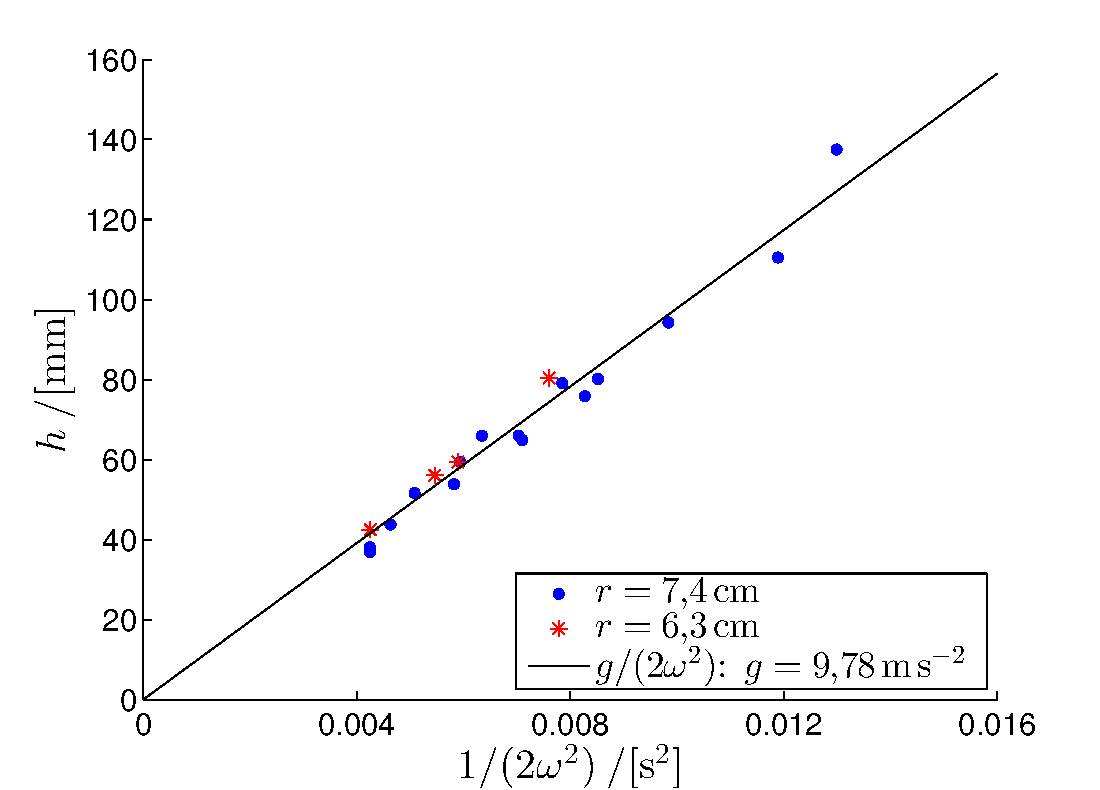
\includegraphics[width=.7\textwidth]{g_minsta_kvadrat.pdf}
\caption{\label{fig:data_vattenparabel} Mätpunkter för olika fokushöjder (med korrektion för mätning vid sidan om centrum) och rotationshastigheter tillsammans med en minsta kvadrat-anpassad kurva (anpassningen är gjord efter alla mätpunkter). Mätningar är gjorda för två olika radiella avstånd mellan rotationsaxel och infallande laserstråle, $r$ i \figref{fig:rot_bowl}.
Eftersom $h=g/(2\omega^2)$ gäller det att $g$ är lutningen till kurvan.}
\end{figure}

\subsection{Bestämning av Newtons gravitationskonstant}
Vinkeln $\varphi$ som funktion av tid visas i \figref{fig:phi} för två olika värden på $\alpha$. En minsta kvadrat-anpassning har gjorts till funktionen
\begin{equation}
\widehat\varphi(t) = A\exp(-Bt)\sin(\omega t+C)+D,
\label{eq:phianpassning}
\end{equation}
med $A=0,032$, $B=1,0\times 10^{-3}$\,s$^{-1}$, $C=0,9$, $D=0,021$ och $\omega=9,8\times10^{-3}$\,s$^{-1}$. Torsionspendelns tröghetsmoment utifrån mätningarna av periodtid vid inverkan av gravitationen var $2,4\times10^{-4}$\,kg\,m$^2$. Om samma tröghetsmoment beräknas utifrån antagandet att all massa är centrerad i blykloten blir motsvarande värde $1,1\times10^{-4}$\,kg\,m$^2$. Det senare är en övre begränsning av det korrekta värdet, och om detta används för i kombination med $\omega$ ur ekvation \eqref{eq:phianpassning} blir $k=1,0\times10^{-8}$\,Nm. Ur ekvation~\eqref{eq:Gformel} erhölls sedan värden på $G$ enligt Tabell~\ref{tab:G}. Det slutliga värdet på $G$, givet av medelvärdet samt maxfelet, blir alltså $G=\unit[(8\pm2)\times 10^{-11}]{N\,m^2\,kg^{-2}}$.

\begin{figure}%[H]
\centering
\includegraphics[width=0.7\textwidth]{phi.eps}
\caption{Svängningsförloppet för torsionspendeln vid två olika värden på $\alpha$. Vinkeln $\varphi$ som funktion av tiden kan anpassas väl av en dämpad sinuskurva $\widehat\varphi(t)$.}
\label{fig:phi}
\end{figure}

\begin{table}%[H]
\centering
\caption{Uppmätta värden på Newtons gravitationskonstant $G$ för olika vinklar $\alpha$ hos vridarmen med de stora blykloten i \figref{fig:cavendish}.}
\begin{tabular}{|c|c|c|c|c|} \hline
$\alpha$ & 130$^\circ$ & 49$^\circ$ & 70$^\circ$ & 110$^\circ$ \\ \hline
$G$/[10$^{-11}$\,N\,m$^2$\,kg$^{-2}$] & 7,23 & 9,19 & 10,0 & 5,67 \\ \hline  
\end{tabular}
\label{tab:G}
\end{table}




\section{Diskussion}
Överlag verkar resutaten från tyngdaccelerationen ge förväntade resultat -- de stämmer överens, både med varandra och med tabellvärden. För mätningen av $g$ med vattenparabeln blev resultaten till och med över förväntan.

Mätningen av Newtons gravitationskonstant var inte lika nära det tabulerade värdet. Men med tanke på den stora spridningen i mätningarna är felet i våra mätningar så stort att det i nuläget kan anses meningslöst att  försöka hitta systematiska fel i den uppmätta datan.

\subsection{Reversionspendel}
Resultaten från mätningarna av periodtiden med kamerasystemet respektive fotodioden är nätt och jämnt inom varandras osäkerheter, även då de båda metoderna användes samtidigt. En möjlig anledning kan vara att kamerasystemets klocka gick något för fort. Fotodioden och oscilloskopet (vars klocka antogs vara mer noggrann) användes för att mäta kamerornas samplingsfrekvens men eftersom felmarginalen var så stor gick det inte att bevisa att $f_s>100$\,Hz. Även en samplingsfrekvens på 100,002 Hz ger en korrektion till $T$ på $\Delta T/T = 2\times 10^{-5}$, vilket är försumbart vid sidan av $\Delta d/d$.

Noggrannheten begränsas alltså av mätningen av $d$. Skjutmåttet har idealt en osäkerhet på 0,05\,mm, men det gick att vicka lite på skänklarna och vi behövde laga det själva eftersom vissa skruvar satt fel. Dessutom var det för kort för att mäta avstånd över en meter, vilket gjorde att ett annat skjutmått behövde användas för att göra kompletterande mätningar, vilket leder till ytterligare fel. Därför litar vi inte på mätningen till mer än 0,5\,mm. Det enklaste sättet att förbättra detta är att skaffa ett längre och mindre slitet skjutmått. 

Värdet på tyngdaccelerationen vid Chalmers är 9,8172\,m\,s$^{-2}$ enligt Bureau Gravimétrique International\cite{BGI:reference}. Detta är inom felmarginalen för det uppmätta värdet, om än i underkant. Eventuellt finns alltså något systematiskt fel som överskattar $g$, till exempel att skjutmåttet ger ett för litet värde på $d$. Pendeln är inte heller helt symmetrisk i sin form kring mittpunkten, så att korrektionen för lyftkraft kan inte försummas helt.

En annan möjlig felkälla är att upphängningseggarna inte nödvändigtvis var helt parallella. Stångens tröghetsmoment med avseende på de olika axlarna följer då inte längre Steiners sats. Detta bör ha liten påverkan, eftersom pendeln var nära cylindriskt symmetrisk, med undantag för vikterna. Det är dock utanför denna rapports omfång att kvantitativt beräkna korrektionen för detta.

%Det fanns även två mindre vikter (en av mässing och en av aluminium), men dessa hittades inte förrän laborationstiden var slut. Dessa hade kunnat användas för att finjustera periodtiderna utan att behöva flytta eggarna eller de stora vikterna.


%Det korrekta värdet på tyngdaccelerationen, vid havsnivån, varierar med latituden $\phi$ enligt
%\[ g = (1+5,2790414\sin^2\phi + 2,32718\sin^4\phi) \times 9,780327 \mathrm{m\,s}^{-2}, \]
%med lokala variationer av storleksordningen 10$^{-}$ m\,s$^{-2}$ \cite{kater}.

\subsection{Vattenparabel}
Utgångspunkten för de här mätningarna var att metoden troligen skulle vara så onoggrann att osäkerheten i mätningarna skulle ligga kring 10~\% på grund av svårigheter att lokalisera fokus och krusningar på vattenytan. Under mätningarna visade det sig dock att reflektionen efter ett par minuter hade stabiliserats. Fokus kunde sedan tämligen enkelt bestämmas. Det visade sig att mätmetoden med vattenparabeln gav en osäkerhet på $\unit[0,1]{m\,s^{-2}}$ vilket motsvarar en relativ osäkerhet på cirka 1~\%. 


\subsubsection{Begränsningar i rotationshastighet}
Som \figref{fig:data_vattenparabel} visar har mätningarna gjorts i ett ganska snävt intervall av rotationshastigheter. Det hade såklart varit önskvärt att försöka göra mätningar i ett större intervall men det var tyvärr inte möjligt. Rotationshastigheten begränsades uppåt av att vatten börjarde spilla ut ur den roterande skålen vid för högt $\omega$, notera att detta motsvarar en \emph{nedre} begränsning på $1/(2\omega^2)$ i \figref{fig:data_vattenparabel}. 

Rotationshastigheten begränsades nedåt på grund av att parabeln blev för flack för att kunna göra säkra avläsningar av $\hat{h}$. Ett lågt $\omega$ leder till att vinkeln $2\alpha$ i \figref{fig:rot_bowl} blir väldigt liten, vilket i sin tur gör att en liten osäkerhet i vinkeln blir en mycket större osäkerhet i $\hat{h}$. Och eftersom det hela tiden var små krusningar på vattenytan gav det hela tiden små vinkelvatiationer. Alltså bör man inte göra mätningar vid allt för låga $\omega$ då det ger större osäkerhet. Detta kan eventuellt urskiljas i \figref{fig:data_vattenparabel} för de höga värdena på $1/(2\omega^2)$ då mätpunkterna där ligger mer spritt.

För att kunna höja $\omega$ krävs en djupare skål och en bättre balanserad uppställning. Skålens väggar måste vara högre, med de måste dessutom vara lodräta. Vidare behöver uppställningen balanseras bättre för att minska skakningar på grund av obalans. 

Om mätningar ska göras vid riktigt låga vinkelfrekvenser krävs en mycket stabil uppställning. Krusningarna på vattenytan måste då i mycket högre grad elimineras för att inte orsaka mycket stora osäkerheter i höjdmätningen. 



\subsubsection{Begränsningar i laserns position}

Mätningar gjordes enbart för två olika radiella avstånd mellan den infallande laserstrålen och rotationsaxeln, $r$ i \figref{fig:rot_bowl}. Det kan tyckas vara en svaghet, men $r$ ska inte påverka värdet på $g$ eftersom alla lodrätt infallande ljusstrålar kommer att reflekteras till paraboloidens fokus. Vidare finns även en del praktiska svårigheter med att variera $r$ allt för mycket. %Vidare var det praktiskt svårt att komma åt att mäta $\hat{h}$ för små $r$. Det gick heller inte att ha allt för stora $r$ då det ledde till att laserstrålen inte träffade vattenytan annat än för höga $\omega$. 
Dock gjordes ändå mätningar för två olika $r$. 

Som kan ses i \figref{fig:data_vattenparabel} ser det ut som om mätningarna med $r=\unit[6,3]{cm}$ systematiskt ligger över den anpassade kurvan. Detta är lite märkligt eftersom det teoretiskt inte borde ge någon påverkan. Det kan bero på att krusningarna var värre nära skålens centrum på grund av att centralstaven som stod i vattnet. Det går heller inte att utesluta att det bara var slumpmässiga fel som råkade sammanfalla i just de fyra mätningarna. Det skulle behövas fler mätningar i den mätserien för att kunna avgöra detta.

\subsubsection{Alternativa tillvägagångsätt}
För att minska krusningarna på vattenytan använde Berg\cite{Berg1990} och IPhO\cite{IPhO2001} glycerol istället för vatten. Eftersom glycerol har en mycket högre viskositet än vatten kommer en sådan uppställning inte få lika mycket krusningar på vattenytan.
Detta skulle kunna öka noggrannheten betydligt då de största osäkerheterna kommer från avläsning av fokus ligger. I vårt fall fanns det faktiskt glycerol tillgängligt, men då skålen som användes i experimentet egentligen var en skål från ett kök och var avsedd för livsmedel ansågs det olämpligt att använda glycerol.

Ett annat sätt att minska krusningarna kan eventuellt vara att mäta fokushöjden, $h$ på ett sätt som inte involverar en centralstav som sticker ner i vattnet. Till exempel skulle $h$ kunna mätas med två lodräta laserstålar. De två laserstrålarna skulle då korsa varandra i fokus. Detta kräver dock att båda lasrarna är väldigt välriktade från början.

\v{S}abatka och Dv\v{o}rák\cite{Sabatka2010} använde sig av en uppställning med flera metallstavar på rad som fästes så att de följde vattenytan. På så sätt kan de sedan anpassa en andragradskurva efter metallstavarna nedsänkning. Denna metod skulle eventuellt kunna ge ett noggrannare värde på $g$, men dess stora nackdel är att den kräver specialtillverkad utrustning. 


\subsection{Cavendish-pendel}\label{sec:cavkorr}
Bestämningen av $I$ utifrån antagandet att all torsionspendelns massa är koncentrerad i blyklotens centrum,

Eftersom torsionspendelns svängning är dämpad är det uppmätta värdet på $\omega$ något förskjutet från $\omega_0=\sqrt{k/I}$. Rörelseekvationen för en linjärt dämpad fjäder med dämpningskoefficient $c$ är
\[ \ddot \varphi + \frac{c}{I}\dot \varphi + \frac{k}{I}\varphi = 0,\]
med lösning $\phi=A\exp\left(-\frac{c}{2I}t\right)\sin(\omega t+C)+D$, där 
$\omega =\sqrt{\frac{k}{I}-\left(\frac{c}{2I}\right)^2}$. Alltså är
\[k = I\left( \omega^2+\left(\frac{c}{2I}\right)^2 \right). \]
Ur anpassningen i ekvation \eqref{eq:phianpassning} erhålles härigenom $\Delta k/k = 0,01$, varför detta fel kan anses vara försumbart.

Det tabulerade värdet på $G$ ligger inom felmarginalerna, som är så stora att vidare överläggningar om små korrektioner blir onödiga. Metoden begränsas huvudsakligen av svårigheten att mäta $\alpha$. Ett sätt att förbättra detta vore att även på vridarmen sätta upp en liten spegel som en egen laser kan riktas mot. En annan svårighet är att noga avläsa laserprickens position vid bestämningen av $\phi$. Genom att använda en lins för att kollimera lasern bör denna osäkerhet kunna minskas.

\section{Slutsatser}
%\textcolor{red}{Vi förtjänar glass!}\\
Som väntat erhölls ett noggrannare värde på $g$ från reversionspendeln än från vattenparabeln. Med reversionpendeln kunde tyngdaccelerationen bestämmas med tre värdesiffror. Det största bidraget till osäkerhet i den här metoden var avståndsmätningen mellan upphängningspunkterna.

Men även mätningen med vattenparabeln visade sig kunna ge ganska noggranna mätningar av tyngdaccelerationen -- dock var osäkerheten fortfarande mer än 10 gånger större än för reversionspendeln. 
I och med den här rapporten går det alltså att konstatera att denna hittills, så vitt vi vet, obeprövade metod verkar fungera. %I grova drag gick metoden ut på att bestämma $g$ genom att finna fokus från vattenytan i en roterande skål.
Metoden kräver dock en mycket stabil uppställning för att eliminera krusningar på vattenytan. Detta torde vara metodens största svaghet. I övrigt kan den här metoden anses som en ganska enkel metod som inte kräver särskilt avancerad teori.

För mätningen av $G$ erhölls ett värde där det tabulerade värdet på $G$ ligger inom felmarginalen för denna mätning. Dock får den relativa osäkerheten på 25\,\% anses vara ganska stor. Det var dock väntat då det var en ganska liten uppställning som användes. 










%Nudu Runeson! Du ville ha ett sätt att sortera referenser efter ordningen som de används. Här har du det. Gör såhär om du vill lägga in referenser:
%Gå in i 'delC.bib'. Där finner du två referenser som jag har lagt in.
%Följ samma mönster som jag har använt.
%Det först ordet är det som \cite använder.
%(\cite använder du som vanligt här i texten.)
\iflanguage{swedish}{\renewcommand{\refname}{Källförteckning}}{}
\bibliographystyle{babunsrt}
\bibliography{delC}
%Gör inget dumt nu. Vill du lägga till referenser så gör det på dethär sättet.



\clearpage
\appendix
\setcounter{page}{1}
\renewcommand*{\thepage}{A\arabic{page}}
\phantomsection{}
\addcontentsline{toc}{part}{Bilagor}



\section{Teoribakgrund}
För den intresserade finns här utförligare förklaringar och härledningar av olika koncept i texten. 

\subsection{Reversionspendel}
En fysikalisk pendel med massan $m$ har en rörelseekvation given av \cite{beckman}
\[ \ddot\theta + \frac{mgl}{I}\sin\theta = 0,\]
där $l$ är avståndet mellan rotationsaxeln och masscentrum och $I$ tröghetsmomentet med avseende på denna axel. Svängningsfrekvensen för små svängningar ges av 
\begin{equation}
\omega^2 = \frac{gml}{I},
\label{omega}
\end{equation}
 Enligt Steiners sats gäller $I=I_0+ml^2$, där $I_0$ är tröghetsmomentet med avseende på en parallell rotationsaxel genom masscentrum. Nu kan $l$ lösas ut enligt \cite{kater}

\begin{equation}
l=\frac{g}{2\omega^2}\pm\sqrt{\frac{g^2}{4\omega^4}-\frac{I_0}{m}}.
\label{katerekv}
\end{equation}
Det finns alltså två rotationsaxlar som ger varje given periodtid, på varje sida av masscentrum (varje positivt avstånd $l$ svarar mot en rotationsaxel på vardera sida om masscentrum). Välj nu lösningen $l=\frac{g}{2\omega^2}+\sqrt{\frac{g^2}{4\omega^4}-\frac{I_0}{m}}$ på ena sidan och $l'=\frac{g}{2\omega^2}-\sqrt{\frac{g^2}{4\omega^4}-\frac{I_0}{m}}$ på andra sidan. Avståndet mellan dessa båda rotationsaxlar blir då $l+l'=\frac{g}{\omega^2}\equiv d$, så att kvadratrotsuttrycket försvinner och $d$ blir oberoende av rotationskroppens massfördelning. Genom att identifiera avståndet $d$ mellan dessa axlar och mäta vinkelfrekvensen $\omega$ kan $g$ beräknas noga ur
\[g= \omega^2d.\]
Med denna metod behöver alltså pendelns massfördelning inte vara känd.

\subsubsection{Korrektioner}\label{sec:katerkorr}
I allmänhet kommer pendelns periodtid att behöva korrigeras för luftmotstånd och för lyftkraft från luften. Om pendelns form är symmetrisk kring punkten mitt emellan upphäningspunkterna kommer dock dessa korrektioner att bli noll \cite{kater}. Detta är dock inte fallet i den metod som används i denna studie. Lyftkraften från luften är motriktad gravitationen, vilket medför en minskning av den effektiva massan, som minskar det vridande momentet från tyngdkraften med $m_\mathrm{luft}gl\sin\theta$ och därmed även minskar svängningsfrekvensen. Korrektionen i periodtid $T$ blir $\frac{\Delta T}{T}= \frac{m_\mathrm{luft}}{2m}$. Här betecknar $m_\mathrm{luft}$ massan hos den luft som trängs undan av pendelkroppen. Om pendelns beståndsdelar är gjord av material med olika densitet behöver dessas delars bidrag beräknas separat.

Ekvation~\eqref{omega} ovan bygger på antagandet om små utslagsvinklar i lösningen av $\ddot\theta + \frac{mgl}{I}\sin\theta=0$. Om maximala utslagsvinkeln är $\theta_0$ ges den exakta lösningen av en elliptisk integral, som ger en korrektion till periodtiden $T=2\pi/\omega$ enligt \cite{planpendel1986}
\begin{equation} \label{eq:korr}
\frac{\Delta T}{T} = \frac{1}{16}\theta_0^2 + \frac{11}{3072}\theta_0^2 + \dots
\end{equation}
Denna formel behöver modifieras för att ta hänsyn till dämpningens påverkan på periodtiden, som orsakas av luftmotstånd och friktion. I fallet linjär dämpning blir denna
\[ \frac{\Delta T_\text{linjär}}{T} = \frac{\theta_{0i}^2 - \theta_{0f}^2}{32\ln(\theta_{0i}/\theta_{0f})}, \]
där $\theta_{0i}$ och $\theta_{0f}$ betecknar initiala respektive slutliga amplituden. I fallet kvadratisk dämpning blir korrektionen istället
\[ \frac{\Delta T_\mathrm{kvadratisk}}{T} = \frac{1}{16}\theta_{0i}\theta_{0f}. \]
Den slutliga korrektionen kan beräknas genom att summera avvikelserna från ekvation~\eqref{eq:korr} i fallen linjär respektive kvadratisk dämpning och sedan använda denna summa som den verkliga avvikelsen från~\eqref{eq:korr}.\cite{planpendel1986}







\subsection{Vattenparabel}\label{sec:vattenparabel_teori}
%Om en cirkulär skål med vatten roteras kring sin mittpunkt kommer vattenytan att bilda en rotationsparaboloid. Paraboloidens form kommer då enbart att bero på rotationshastigheten, $\omega$, och tyngdaccelerationen, $g$.

Ett enkelt sätt att visa att vattenytan kommer att bli en rotationsparaboloid är att betrakta vinkeln $\alpha$ i \figref{fig:vatten}. Beteckna vattenytans höjd över paraboloidens vertex (dess bottennivå) $z(r)$. Då gäller att 
\begin{equation*}
\tan\alpha = \frac{\rd z}{\rd r},
\end{equation*}
men det går även att uttrycka $\tan\alpha$ med centrifugalaccelerationen $a_c=r\omega^2$ och $g$ vilket ger:
\begin{equation}\label{eq:lutning}
\frac{\rd z}{\rd r}%=\frac{a_c}{g}
=\tan\alpha =\frac{r\omega^2}{g}.
\end{equation}
Detta ger nu slutligen
\begin{equation*}
z(r)
=\frac{r^2\,\omega^2}{2g}.
\end{equation*}
%Notera att integrationskonstanten blir 0 då $z(r)$ definieras som höjden över paraboloidens vertex.
Detta är en parabel och dess fokus ligger på höjden\cite{Physics_Handbook}
\[ h=\frac{g}{2\omega^2} \]
över vertex.

\begin{figure}\centering
\input{vattenparabel.pdf_t}
\caption{\label{fig:vatten} Tvärsnitt av vattenyta i en roterande skål. Varje element av vattenytan kommer alltid att vara vinkelrät mot den totala (inkluderande fiktiva) accelerationen på ytelementet. Detta betyder att om en cirkulär skål med vatten roteras kring sin symmetriaxel kommer vattenytan i skålen att bilda en rotationsparaboloid.}
\end{figure}

\subsubsection{Korrektion för mätning vid sidan om rotationsaxeln}
Som \figref{fig:rot_bowl} visar kommer man behöva göra en korrektion av den uppmätta höjden $\hat{h}$för att den mäts utanför rotationsaxeln. 

Vi börjar med att konstatera att korrektinen blir
\[ \delta = \rho \cot{2\alpha}, \]
dock behöver vinkeln $\alpha$ bestämmas. För att göra detta kan vi konstatera att 
\[ \cot{2\alpha} = \frac{\hat{h}-z(r)}{\hat{r}} = \frac{\hat{h}}{\hat{r}} - \frac{r^2\omega^2}{2g\hat{r}}. \]
Med hjälp av \eqref{eq:lutning} kan vi nu ersätta den sista termen i högerledet till
\[ \cot{2\alpha} =  \frac{\hat{h}}{\hat{r}} - \frac{r}{2\hat{r}}\tan{\alpha} \]
vilket är en omskrivning av \eqref{eq:vinkelekvation} i avsnitt~\ref{sec:vattenparabel_korrektion}.



\subsection{Newtons gravitationskonstant}\label{sec:cavendish}
Med uppställningen i~\figref{fig:cavendish} kan momentet på \emph{ett} av de upphängda kloten med avseende på upphängningspunkten, $O$, beräknas. Först beräknas krafterna på ett blyklot:
\begin{equation*}
\begin{aligned}
F_1&=G\frac{m_1 m_2}{d_1^2}\\
F_2&=G\frac{m_1 m_2}{d_2^2},
\end{aligned}
\end{equation*}
där $d_1^2=R^2+r^2-2rR\cos\alpha$ och $d_2^2=R^2+r^2+2rR\cos\alpha$ enligt cosinussatsen.
%Notera här att geometrin i problemet begränsar $\alpha\le 45^\circ$. Så vi kan inte 
Momentet med avseende på $O$ från en av massorna $m_1$ blir:
\begin{equation*}
\begin{aligned}
M_1&=F_1 r\sin{\beta}=F_1 \frac{rR}{d_1}\sin\alpha\\
M_2&=-F_2 r\sin{\gamma}=-F_2 \frac{rR}{d_2}\sin\alpha,
\end{aligned}
\end{equation*}
där de sista likheterna följer av sinussatsen. Det totala momentet med avseende på $O$ från båda massorna blir nu:
\begin{equation}\label{eq:moment}
\begin{aligned}
M=&2(M_1+M_2)=\\
 =& 2G m_1 m_2 r R \sin\alpha
%\frac{\cos{\alpha}^3-\sin{\alpha}^3}{\sin{\alpha}^2\cos{\alpha}^2}.
\left( \frac{1}{(R^2+r^2-2rR\cos\alpha)^{3/2}} - \frac{1}{(R^2+r^2+2rR\cos\alpha)^{3/2}} \right)\\
M=& k\varphi.
\end{aligned}
\end{equation}
Härur kan nu $G$ bestämmas om man har massorna, vinklarna, radierna och fjäderkonstanten.

Vidare gäller att vinkeländringen $\varphi$ kan mätas med laserreflektion som till vänster i \figref{fig:cavendish}. Fördelen med att mäta vinkeln mellan reflekterade strålar är att den vinkeländringen $\Delta\theta=2\varphi$. Alltså erhålls dubbelt så stort vinkelutslag på reflektionen.





\begin{comment}
\subsubsection{Vinklarna i Cavendishs experiment}\label{sec:vinklar}
För att beräkna alla vridmoment i experimentet behöver vi finna de olika vinklarna som förekommer. I \figref{fig:cavendish_geometri} visas ett sätt att finna vinkeln $\angle{OCB}$ kan man använda randvinkelsatsen. Det antas här att vinkeln $\angle{AOC}$ kan mätas ur experimentet. 

Börja med att konstatera att alla klotens masscentrum ligger på en cirkel med centrum i punkten $O$. Då gäller enligt randvinkelsatsen att 
\[\angle{ABC}=\frac{1}{2}\angle{AOC}.\]
Vidare gäller att 
\[\angle{OCB}=\angle{OBC}\]
ty de är basvinklar i en likbent triangel\footnotemark. Vi kan härav se att 
\[\angle{OCB}=\frac{1}{2}\angle{AOC}\]
vilket var vad vi skulle finna. 
\footnotetext{Vi har nämligen att $|OC|=|OB|=r$. }

\begin{figure}\centering
\input{cavendish_geometri.pdf_t}
\caption{\label{fig:cavendish_geometri} Vinklarna i Cavendishs experiment kan enkelt finnas genom att använda randvinkelsatsen. }
\end{figure}
\end{comment}


\end{document}


%% På svenska ska citattecknet vara samma i både början och slut.
%% Använd två apostrofer (två enkelfjongar): ''.

%%För att referera till till tidigare fotnot:
%    \footnotemark[\value{footnote}]

%% Figurer inkluderade som pdf-filer
%\begin{figure}\centering
%\centerline{ %centrerar även större bilder
%\includegraphics[width=1\textwidth]{filnamn.pdf}
%}
%\caption{\label{figuren} Perioden $T$ som funktion av pendellängden.}
%\end{figure}

%% Figurer inkluderade med xfigs "Combined PDF/LaTeX"
%\begin{figure}\centering
%\input{filnamn.pdf_t}
%\caption{\label{finafiguren} Perioden $T$ som funktion av
%  pendellängden.}
%\end{figure}



ATT GÖRA
